\subsection{Pokrytí případy užití}
Z tabulky \ref{tab:func_req_uc_table} je vidět, že všechny funkční požadavky na aplikaci jsou pokryty případy užití a tedy, že se na žádnou část nezapomnělo. V přiloženém obrázku \ref{fig:use_case} jsou znázorněni jednotliví aktéři, vztahy mezi nimi a vztahy k případům užití.

\begin{table}
    \centering
    \begin{tabular}{l|l|l|l|l|l|l|l|l|l|l}
             & \rotatebox[origin=c]{90}{PU01} & \rotatebox[origin=c]{90}{PU02} & \rotatebox[origin=c]{90}{PU03} & \rotatebox[origin=c]{90}{PU04} & \rotatebox[origin=c]{90}{PU05} & \rotatebox[origin=c]{90}{PU06} & \rotatebox[origin=c]{90}{PU07} & \rotatebox[origin=c]{90}{PU08} & \rotatebox[origin=c]{90}{PU09} & \rotatebox[origin=c]{90}{PU10} \\
        \hline
        FP01 & x                              &                                & x                              & x                              &                                &                                &                                &                                &                                &                                \\
        \hline
        FP02 &                                & x                              & x                              & x                              &                                &                                &                                &                                &                                &                                \\
        \hline
        FP03 &                                &                                & x                              & x                              &                                &                                &                                &                                &                                &                                \\
        \hline
        FP04 &                                &                                &                                &                                & x                              &                                &                                &                                &                                &                                \\
        \hline
        FP05 &                                & x                              &                                &                                &                                &                                &                                &                                &                                &                                \\
        \hline
        FP06 &                                & x                              &                                &                                &                                &                                &                                &                                &                                &                                \\
        \hline
        FP07 &                                &                                &                                & x                              &                                &                                &                                &                                &                                &                                \\
        \hline
        FP08 &                                &                                &                                &                                &                                &                                &                                &                                &                                & x                              \\
        \hline
        FP09 &                                &                                &                                &                                &                                &                                &                                &                                & x                              &                                \\
        \hline
        FP22 &                                &                                &                                &                                &                                &                                &                                &                                & x                              &                                \\
        \hline
        FP23 &                                &                                &                                &                                &                                &                                & x                              &                                &                                &                                \\
        \hline
        FP24 &                                &                                &                                & x                              &                                &                                &                                &                                &                                &                                \\
        \hline
        FP41 &                                &                                &                                &                                &                                & x                              &                                &                                &                                &                                \\
        \hline
        FP42 &                                &                                &                                &                                &                                & x                              &                                &                                &                                &                                \\
        \hline
        FP61 &                                &                                &                                &                                &                                &                                &                                & x                              &                                &
    \end{tabular}
    \caption{Kontrola pokrytí funkčních požadavků případy užití}
    \label{tab:func_req_uc_table}
\end{table}


\begin{figure}
    \centering
    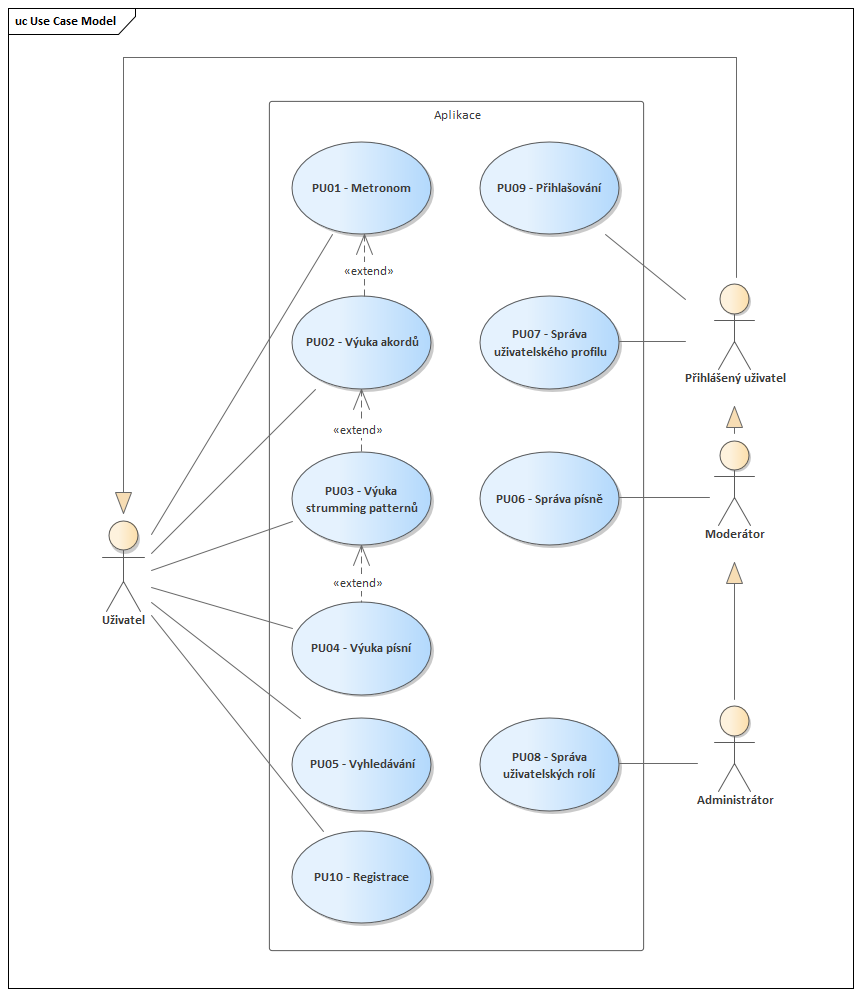
\includegraphics[width=0.9\textwidth]{assets/use_case_model.png}
    \caption{Diagram případu užití}
    \label{fig:use_case}
\end{figure}